\documentclass[11pt]{article}
\usepackage[T1]{fontenc}
\usepackage{lmodern}
\usepackage[a4paper,left=25mm,right=30mm,top=22mm,bottom=24mm,marginparwidth=18mm]{geometry}
\usepackage{amsmath,amssymb,mathtools,stmaryrd}
\usepackage{tikz}
\usetikzlibrary{arrows.meta,calc,positioning}
\usepackage{caption}
\usepackage{xcolor}
\usepackage{marginnote}
\usepackage{microtype}
\usepackage{needspace}
\usepackage[hidelinks]{hyperref}
\definecolor{LeanTeal}{HTML}{087F72}
\definecolor{SourceGray}{HTML}{66736F}
\setlength{\parindent}{0pt}
\setlength{\parskip}{0.55em}
\setlength{\emergencystretch}{2em}
\newcommand{\leanmarker}[2]{%
  \Needspace{3\baselineskip}%
  \marginnote{\hyperlink{#1}{\color{LeanTeal}\fbox{\scriptsize Lean}}}%
  \hypertarget{#1}{\textbf{#2.}}%
}
\newcommand{\sourcepage}[1]{\par\medskip\noindent\textcolor{SourceGray}{\scriptsize Source PDF page #1}\par\smallskip}
\pagestyle{plain}
\begin{document}
\begin{center}\LARGE\bfseries Recursive domain equations\par\medskip
\large Lean 4 Formalization Companion -- Chapter 5\end{center}
\medskip
\noindent\textit{This project-generated reading copy contains reviewed mathematical items, short source locators, and redrawn diagrams. It does not reproduce the original PDF or automatic OCR prose. Click a Lean tag in the web reader to open the mapped Lean declaration.}
\bigskip\hrule\bigskip
\section*{Section 5.1}
\sourcepage{69}
\leanmarker{def-5-1-1}{Definition 5.1.1} Let \(F\) be a functor on a category \(\mathbf C\). An \(F\)-algebra is an object \(A\) together with a map \(f:F(A)\to A\). A homomorphism from \(f:F(A)\to A\) to \(f':F(A')\to A'\) is a map \(g:A\to A'\) such that
\[
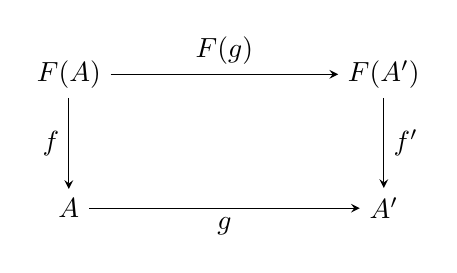
\begin{tikzpicture}[baseline=(current bounding box.center), >=stealth]
  \node (FA)  at (0,1.7) {$F(A)$};
  \node (FAp) at (4.0,1.7) {$F(A')$};
  \node (A)   at (0,0) {$A$};
  \node (Ap)  at (4.0,0) {$A'$};
  \draw[->] (FA) -- node[above] {$F(g)$} (FAp);
  \draw[->] (FA) -- node[left] {$f$} (A);
  \draw[->] (FAp) -- node[right] {$f'$} (Ap);
  \draw[->] (A) -- node[below] {$g$} (Ap);
\end{tikzpicture}
\]
commutes.

\leanmarker{lemma-5-1-2}{Lemma 5.1.2} If \(i:F(A)\to A\) is an initial \(F\)-algebra, then \(i\) is an isomorphism.
\emph{Proof sketch.} Let \(f\) be the unique homomorphism from \(i:F(A)\to A\) to \(F(i):F^2(A)\to F(A)\). The proof uses the composition of homomorphisms displayed below:
\[
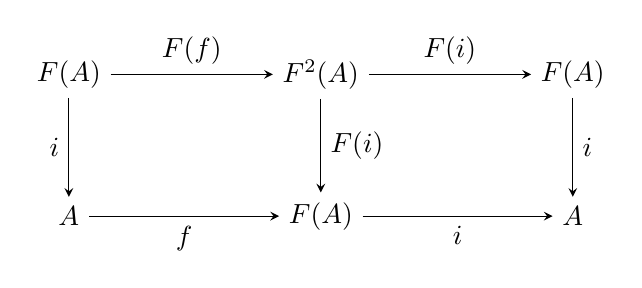
\begin{tikzpicture}[baseline=(current bounding box.center), >=stealth]
  \node (FA0) at (0,1.8) {$F(A)$};
  \node (F2A) at (3.2,1.8) {$F^2(A)$};
  \node (FA1) at (6.4,1.8) {$F(A)$};
  \node (A0)  at (0,0) {$A$};
  \node (FA2) at (3.2,0) {$F(A)$};
  \node (A1)  at (6.4,0) {$A$};
  \draw[->] (FA0) -- node[above] {$F(f)$} (F2A);
  \draw[->] (F2A) -- node[above] {$F(i)$} (FA1);
  \draw[->] (FA0) -- node[left] {$i$} (A0);
  \draw[->] (F2A) -- node[right] {$F(i)$} (FA2);
  \draw[->] (FA1) -- node[right] {$i$} (A1);
  \draw[->] (A0) -- node[below] {$f$} (FA2);
  \draw[->] (FA2) -- node[below] {$i$} (A1);
\end{tikzpicture}
\]
Initiality gives \(i\circ f=\operatorname{id}_A\), and the remaining equality gives the inverse law on \(F(A)\).

\clearpage
\section*{Section 5.2}
\sourcepage{70}
\leanmarker{def-5-2-1}{Definition 5.2.1} A functor \(F:\mathbf{D}^e\to\mathbf{D}^e\) is continuous if, for every expanding sequence \(\langle(D_n)_{n\in\mathbb N},(e_{mn}:D_n\to D_m)_{n\le m}\rangle\) with colimit \(\langle D,(e_n)_{n\in\mathbb N}\rangle\), the cocone
\[
  \langle F(D),(F(e_n))_{n\in\mathbb N}\rangle
\]
is a colimit of the sequence \(\langle(F(D_n))_{n\in\mathbb N},(F(e_{mn}))_{n\le m}\rangle\).

\sourcepage{71}
\leanmarker{lemma-5-2-2}{Lemma 5.2.2} Let \(F\) be a continuous functor on a category \(\mathbf{D}^e\) of domains. For an embedding \(e:A\to F(A)\), let \(\langle D,(e_n)_{n\in\mathbb N}\rangle\) be the colimit of
\[
  A\xrightarrow{e}F(A)\xrightarrow{F(e)}F(F(A))\xrightarrow{F(F(e))}\cdots.
\]
Then \(D\cong F(D)\). The isomorphism is given by
\[
\begin{aligned}
\operatorname{fold}&=\bigvee_{n\in\mathbb N} e_{n+1}\circ F(e_n)^*:F(D)\to D,\\
\operatorname{unfold}&=\bigvee_{n\in\mathbb N}F(e_n)\circ e_{n+1}^*:D\to F(D),
\end{aligned}
\]
and for every \(n\),
\[
  F(e_n)=\operatorname{unfold}\circ e_{n+1},\qquad
  F(e_n)^*=e_{n+1}^*\circ\operatorname{fold}.
\]

\leanmarker{def-5-2-3}{Definition 5.2.3} A functor \(F:\mathbf D\to\mathbf E\) between categories of domains is called locally continuous if, for every pair of objects \(D,D'\), the map
\[
  \operatorname{Hom}(D,D')\longrightarrow\operatorname{Hom}(F(D),F(D')),
  \qquad f\longmapsto F(f),
\]
is Scott-continuous.

\leanmarker{prop-5-2-4}{Proposition 5.2.4} A locally continuous functor \(F:\mathbf D\to\mathbf E\) restricts to a continuous functor \(F:\mathbf D^e\to\mathbf E^e\) on the corresponding categories of embeddings.

\sourcepage{72}
\leanmarker{def-5-2-5}{Definition 5.2.5} A functor \(F:\mathbf{D}^{op}\times\mathbf{D}'\to\mathbf{E}\), contravariant in the first coordinate and covariant in the second, is locally continuous if, for directed sets \(A\subseteq\operatorname{Hom}(D_2,D_1)\) and \(A'\subseteq\operatorname{Hom}(D'_1,D'_2)\),
\[
  F\bigl(\bigvee{}^{\uparrow}A,\bigvee{}^{\uparrow}A'\bigr)
  =\bigvee{}^{\uparrow}_{f\in A,\,f'\in A'}F(f,f')
\]
in \(\operatorname{Hom}(F(D_1,D'_1),F(D_2,D'_2))\).

\leanmarker{prop-5-2-6}{Proposition 5.2.6} If \(F:\mathbf{D}^{op}\times\mathbf{D}'\to\mathbf{E}\) is mixed-variant and locally continuous, it defines a continuous covariant functor \(\widehat F:\mathbf{D}^e\times\mathbf{D}'^e\to\mathbf{E}^e\) by
\[
  \widehat F(D,D')=F(D,D'),\qquad
  \widehat F(e,e')=F(e^*,e')
\]
for embeddings. The upper adjoint of \(\widehat F(e,e')\) is \(F(e,e'^*)\). If \((e,e^*)\) and \((e',e'^*)\) are embedding-projection pairs, then
\[
\begin{aligned}
F(e,e'^*)\circ\widehat F(e,e')&=F(e,e'^*)\circ F(e^*,e')=F(e^*\circ e,e'^*\circ e')=\operatorname{id},\\
\widehat F(e,e')\circ F(e,e'^*)&=F(e^*,e')\circ F(e,e'^*)=F(e\circ e^*,e'\circ e'^*)\sqsubseteq\operatorname{id}.
\end{aligned}
\]
Thus \(\widehat F\) maps embeddings to embeddings. Continuity follows by applying local continuity to expanding sequences in the two coordinates.

\sourcepage{73}
\leanmarker{prop-5-2-7}{Proposition 5.2.7} Let \(F:\mathbf{D}_{\bot!}\times\mathbf{E}_{\bot!}\to\mathbf{E}_{\bot!}\) be locally continuous. Then the assignment
\[
  D\mapsto \operatorname{FIX}(F_D),\qquad F_D(E)=F(D,E),
\]
extends to a locally continuous functor \(\mathbf{D}_{\bot!}\to\mathbf{E}_{\bot!}\). On a strict map \(f:D\to D'\), the induced map is
\[
  f\mapsto \bigvee_{n\in\mathbb N} e'_n\circ f_n\circ e_n^*,
\]
where \(f_0=\operatorname{id}_{\mathbb I}\) and \(f_{n+1}=F(f,f_n)\). The canonical solution of \(X\cong F(D,X)\) is obtained as the bilimit of
\[
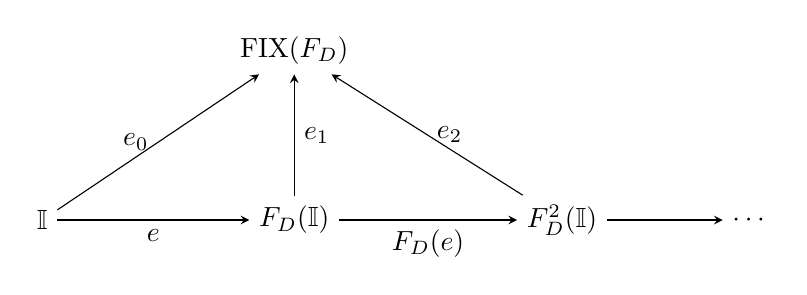
\begin{tikzpicture}[baseline=(current bounding box.center), >=stealth]
  \node (Fix) at (3.2,2.15) {$\operatorname{FIX}(F_D)$};
  \node (I)   at (0,0) {$\mathbb I$};
  \node (FDI) at (3.2,0) {$F_D(\mathbb I)$};
  \node (FD2) at (6.6,0) {$F_D^2(\mathbb I)$};
  \node (Dots) at (9.0,0) {$\cdots$};
  \draw[->] (I) -- node[below] {$e$} (FDI);
  \draw[->] (FDI) -- node[below] {$F_D(e)$} (FD2);
  \draw[->] (FD2) -- (Dots);
  \draw[->] (I) -- node[left] {$e_0$} (Fix);
  \draw[->] (FDI) -- node[right] {$e_1$} (Fix);
  \draw[->] (FD2) -- node[right] {$e_2$} (Fix);
\end{tikzpicture}
\]
and similarly for \(D'\).

\clearpage
\section*{Section 5.3}
\sourcepage{74}
\leanmarker{lemma-5-3-1}{Lemma 5.3.1} Let \(F\) be a locally continuous functor on a category of domains \(\mathbf D\), and let \(i:F(A)\to A\) be an isomorphism. For every \(F\)-algebra \(f:F(C)\to C\) there is a least homomorphism \(h_{C,A}:A\to C\). It is the least fixed point of the functional \(\phi_{C,A}\) on \([A\to C]\) defined by
\[
  \phi_{C,A}(g)=f\circ F(g)\circ i^{-1}.
\]
Least homomorphisms compose: if \(j:F(B)\to B\) is also an isomorphism, then
\[
  h_{C,A}=h_{C,B}\circ h_{B,A}.
\]
\emph{Proof sketch.} The functional \(\phi_{C,A}\) is continuous because \(F\) is locally continuous and composition is continuous. Hence its least fixed point exists as the supremum of the chain starting from \(c_\bot\); induction shows that this point is below every homomorphism and is itself a homomorphism. Composition follows from Lemma 2.1.21 applied to the square whose horizontal map sends \(g\) to \(g\circ h_{B,A}\), giving \(\operatorname{fix}(\phi_{C,A})=\operatorname{fix}(\phi_{C,B})\circ h_{B,A}\).

\sourcepage{75}
\leanmarker{thm-5-3-2}{Theorem 5.3.2} \emph{(Invariance, Part 1)} Let \(F\) be a locally continuous functor on a category of domains \(\mathbf D\), and let \(i:F(A)\to A\) be an isomorphism. The following are equivalent:
\begin{enumerate}
\item \(A\) is isomorphic to the canonical fixpoint \(\operatorname{FIX}(F)\);
\item \(\operatorname{id}_A\) is the least endomorphism of \(A\);
\item \(\operatorname{id}_A=\operatorname{fix}(\phi_{A,A})\), where \(\phi_{A,A}:[A\to A]\to[A\to A]\) is defined by \(\phi_{A,A}(g)=i\circ F(g)\circ i^{-1}\);
\item \(\operatorname{id}_A\) is the only strict endomorphism of \(A\).
\end{enumerate}
\emph{Proof sketch.} For \(D=\operatorname{FIX}(F)\), the least endomorphism is the least fixed point of \(g\mapsto \operatorname{fold}\circ F(g)\circ\operatorname{unfold}\). With the standard embeddings \(e_n:F^n(\mathbb I)\to D\), induction gives \(c_\bot=e_0\circ e_0^*\) and \(\phi^n(c_\bot)=e_n\circ e_n^*\), whose supremum is the identity by Lemma 3.3.8. The equivalence of (2) and (3) is Lemma 5.3.1. For (3) implies (4), Lemma 2.1.21 is applied to the square with \(H(g)=h\circ g\) for a strict endomorphism \(h\), yielding \(\operatorname{id}_A=H(\operatorname{id}_A)=h\). Finally, the homomorphisms between \(A\) and \(\operatorname{FIX}(F)\) compose to the least endomorphisms, hence to identities under (4).

\sourcepage{76}
\leanmarker{thm-5-3-3}{Theorem 5.3.3} \emph{(Minimality, Part 1)} The canonical fixpoint of a locally continuous functor is a sub-domain of every other fixpoint.

\sourcepage{77}
\leanmarker{thm-5-3-4}{Theorem 5.3.4} \emph{(Initiality)} Let \(F:\mathbf D_{\bot!}\to\mathbf D_{\bot!}\) be a locally continuous functor on a category of domains with strict functions. Then \(\operatorname{fold}:F(D)\to D\) is an initial \(F\)-algebra, where \(D\) is the canonical solution to \(X\cong F(X)\).
\emph{Proof sketch.} For a strict algebra \(f:F(A)\to A\), Lemma 5.3.1 gives a homomorphism \(h:D\to A\), and inspection of the construction shows that \(h\) is strict. Uniqueness is proved as in Theorem 5.3.2, using Lemma 2.1.21 on the commutative square
\[
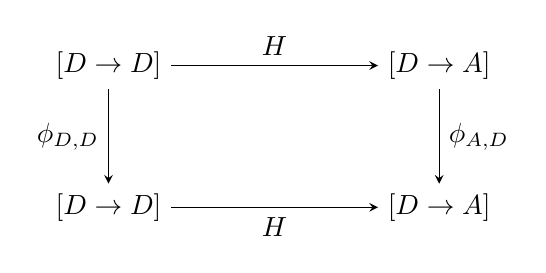
\begin{tikzpicture}[baseline=(current bounding box.center), >=stealth]
  \node (DD0) at (0,1.8) {$[D\to D]$};
  \node (DA0) at (4.2,1.8) {$[D\to A]$};
  \node (DD1) at (0,0) {$[D\to D]$};
  \node (DA1) at (4.2,0) {$[D\to A]$};
  \draw[->] (DD0) -- node[above] {$H$} (DA0);
  \draw[->] (DD1) -- node[below] {$H$} (DA1);
  \draw[->] (DD0) -- node[left] {$\phi_{D,D}$} (DD1);
  \draw[->] (DA0) -- node[right] {$\phi_{A,D}$} (DA1);
\end{tikzpicture}
\]
where \(H(g)=h\circ g\).

\leanmarker{thm-5-3-5}{Theorem 5.3.5} \emph{(Finality)} Let \(F:\mathbf D\to\mathbf D\) be a locally continuous functor with canonical fixpoint \(D=\operatorname{FIX}(F)\). Then \(\operatorname{unfold}:D\to F(D)\) is a final co-algebra.

\leanmarker{lemma-5-3-6}{Lemma 5.3.6} Let \(F:\mathbf D^{op}\times\mathbf D\to\mathbf D\) be a mixed-variant, locally continuous functor, and let \(i:F(A,A)\to A\) and \(j:F(B,B)\to B\) be isomorphisms. Then there exists a least pair of functions \(h:A\to B\) and \(k:B\to A\) such that the two squares
\[
\begin{array}{ccc}
F(A,A)&\xrightarrow{F(k,h)}&F(B,B)\\
\scriptstyle i\downarrow&&\downarrow\scriptstyle j\\
A&\xrightarrow{h}&B
\end{array}
\qquad
\begin{array}{ccc}
F(B,B)&\xrightarrow{F(h,k)}&F(A,A)\\
\scriptstyle j\downarrow&&\downarrow\scriptstyle i\\
B&\xrightarrow{k}&A
\end{array}
\]
commute.

\sourcepage{78}
\leanmarker{thm-5-3-7}{Theorem 5.3.7} \emph{(Invariance, Part 2)} Let \(F:\mathbf D^{op}\times\mathbf D\to\mathbf D\) be a mixed-variant and locally continuous functor, and let \(i:F(A,A)\to A\) be an isomorphism. The following are equivalent:
\begin{enumerate}
\item \(A\) is isomorphic to the canonical fixpoint \(\operatorname{FIX}(F)\);
\item \(\operatorname{id}_A\) is the least mixed endomorphism of \(A\);
\item \(\operatorname{id}_A=\operatorname{fix}(\phi_{A,A})\), where \(\phi_{A,A}:[A\to A]\to[A\to A]\) is defined by \(\phi_{A,A}(g)=i\circ F(g,g)\circ i^{-1}\);
\item \(\operatorname{id}_A\) is the only strict mixed endomorphism of \(A\).
\end{enumerate}
\emph{Proof sketch.} The proof follows Theorem 5.3.2, with the mixed-variance step made explicit. If \(D=\operatorname{FIX}(F)\) and \(e_n:F^n(\mathbb I)\to D\) are the colimiting maps, then the cocone into \(F(D,D)\) gives
\[
  F(e_n^*,e_n)=\operatorname{unfold}\circ e_{n+1},\qquad
  F(e_n^*,e_n)^*=F(e_n,e_n^*)=e_{n+1}^*\circ\operatorname{fold}.
\]
For the least mixed endomorphism, induction gives
\[
\begin{aligned}
\phi^{n+1}(c_\bot)&=\phi(\phi^n(c_\bot))
 =\phi(e_n\circ e_n^*)\\
&=\operatorname{fold}\circ F(e_n\circ e_n^*,e_n\circ e_n^*)\circ\operatorname{unfold}\\
&=\operatorname{fold}\circ F(e_n^*,e_n)\circ F(e_n,e_n^*)\circ\operatorname{unfold}
 =e_{n+1}\circ e_{n+1}^*.
\end{aligned}
\]
Contravariance in the first argument is exactly what swaps \(e_n\) and \(e_n^*\). For (3) implies (4), use Lemma 2.1.21 with \(H(g)=h\circ g\circ h\).

\sourcepage{79}
\leanmarker{thm-5-3-8}{Theorem 5.3.8} \emph{(Minimality, Part 2)} The canonical fixpoint of a mixed-variant and locally continuous functor is a sub-domain of every other fixpoint.

\leanmarker{thm-5-3-9}{Theorem 5.3.9} \emph{(Free mixed-variant algebra)} Let \(F:\mathbf D_{\bot!}^{op}\times\mathbf D_{\bot!}\to\mathbf D_{\bot!}\) be a mixed-variant, locally continuous functor, and let \(D\) be the canonical solution to \(X\cong F(X,X)\). For every pair of strict continuous functions
\[
  f:A\to F(B,A),\qquad g:F(A,B)\to B,
\]
there are unique strict functions \(h:A\to D\) and \(k:D\to B\) such that the two squares
\[
\begin{array}{ccc}
F(B,A)&\xrightarrow{F(k,h)}&F(D,D)\\
\scriptstyle f\uparrow&&\uparrow\scriptstyle\operatorname{unfold}\\
A&\xrightarrow{h}&D
\end{array}
\qquad
\begin{array}{ccc}
F(D,D)&\xrightarrow{F(h,k)}&F(A,B)\\
\scriptstyle\operatorname{fold}\downarrow&&\downarrow\scriptstyle g\\
D&\xrightarrow{k}&B
\end{array}
\]
commute.

\clearpage
\section*{Section 5.4}
\sourcepage{80}
\leanmarker{def-5-4-1}{Definition 5.4.1} A relation \(R\subseteq D^n\) on a pointed domain \(D\) is called admissible if it contains the constantly-bottom tuple and is closed under suprema of \(\omega\)-chains. Write \(\mathcal R^n(D)\) for the set of all admissible \(n\)-ary relations on \(D\), ordered by inclusion; unary relations of this kind are admissible predicates.
If \(f:D\to E\) is strict and continuous, then it acts pointwise on relations by
\[
  f^{rel}(R)=\{\langle f(x_1),\ldots,f(x_n)\rangle\mid \langle x_1,
  \ldots,x_n\rangle\in R\}.
\]

\leanmarker{prop-5-4-2}{Proposition 5.4.2} For dcpo's \(D\) and \(E\), and admissible \(n\)-ary relations \(R\) on \(D\) and \(S\) on \(E\), the set
\[
  \{f\mid f^{rel}(R)\subseteq S\}
\]
is an admissible predicate on the strict function space \([D\to E]\).

\leanmarker{def-5-4-3}{Definition 5.4.3} Let \(F:\mathbf D_{\bot!}^{op}\times\mathbf D_{\bot!}\to\mathbf D_{\bot!}\) be mixed-variant and locally continuous. An admissible action on \(n\)-ary relations for \(F\) is a function \(F^{rel}\) assigning to each pair \(\langle D,E\rangle\) a map
\[
  F^{rel}_{\langle D,E\rangle}:\mathcal R(D)\times\mathcal R(E)
  \to\mathcal R(F(D,E)).
\]
These maps are compatible with strict morphisms as follows: if \(f:D_2\to D_1\), \(g:E_1\to E_2\), \(f^{rel}(R_2)\subseteq R_1\), and \(g^{rel}(S_1)\subseteq S_2\), then
\[
  F(f,g)^{rel}\bigl(F^{rel}_{\langle D_1,E_1\rangle}(R_1,S_1)\bigr)
  \subseteq F^{rel}_{\langle D_2,E_2\rangle}(R_2,S_2).
\]

\sourcepage{81}
\leanmarker{prop-5-4-4}{Proposition 5.4.4} The maps \(F^{rel}_{\langle D,E\rangle}\) are antitone in the first variable and monotone in the second variable.

\leanmarker{thm-5-4-5}{Theorem 5.4.5} Let \(\mathbf D_{\bot!}\) be a category of domains, and let \(F:\mathbf D_{\bot!}^{op}\times\mathbf D_{\bot!}\to\mathbf D_{\bot!}\) be a mixed-variant locally continuous functor with an admissible action on relations. Write \(D=\operatorname{FIX}(F)\). If \(R,S\in\mathcal R^n(D)\) satisfy
\[
  \operatorname{unfold}^{rel}(R)\subseteq F^{rel}(S,R),
  \qquad
  \operatorname{fold}^{rel}\bigl(F^{rel}(R,S)\bigr)\subseteq S,
\]
then \(R\subseteq S\).
\emph{Proof sketch.} By invariance, \(\operatorname{id}_D\) is the least fixed point of \(\phi(g)=\operatorname{fold}\circ F(g,g)\circ\operatorname{unfold}\). Let
\[
  P=\{f\in[D\to D]\mid f^{rel}(R)\subseteq S\}.
\]
This is admissible. If \(g\in P\), then
\[
\begin{aligned}
\phi(g)^{rel}(R)
&=\operatorname{fold}^{rel}\circ F(g,g)^{rel}\circ\operatorname{unfold}^{rel}(R)\\
&\subseteq\operatorname{fold}^{rel}\circ F(g,g)^{rel}\bigl(F^{rel}(S,R)\bigr)\\
&\subseteq\operatorname{fold}^{rel}\bigl(F^{rel}(R,S)\bigr)
 \subseteq S.
\end{aligned}
\]
Thus \(\phi(g)\in P\), so \(\operatorname{id}_D\in P\), which is exactly \(R\subseteq S\).

\leanmarker{def-5-4-6}{Definition 5.4.6} Let \(F\) be a mixed-variant functor as above. An admissible action on \(n\)-ary relations is called logical if, for all objects \(D,E\) and all \(R\in\mathcal R^n(D)\),
\[
  F^{rel}_{\langle D,E\rangle}(R,E^n)=F(D,E)^n.
\]
Specializing Theorem 5.4.5 to \(R=D\) gives the induction principle below.

\leanmarker{thm-5-4-7}{Theorem 5.4.7} \emph{(Induction)} Let \(\mathbf D_{\bot!}\) be a category of domains, and let \(F:\mathbf D_{\bot!}^{op}\times\mathbf D_{\bot!}\to\mathbf D_{\bot!}\) be mixed-variant and locally continuous with a logical action on admissible predicates. Let \(D=\operatorname{FIX}(F)\). If \(S\in\mathcal R^1(D)\) is an admissible predicate such that
\[
  x\in F^{rel}(D,S)\quad\Longrightarrow\quad \operatorname{fold}(x)\in S,
\]
then \(S=D\).
For the primitive constructors, logical actions are given by
\[
\begin{aligned}
R_\bot&=\operatorname{up}(R)\cup\{\bot\}\subseteq D_\bot,\\
R\times S&=\{\langle x,y\rangle\in D\times E\mid x\in R,\ y\in S\},\\
[R\to S]&=\{f\in[D\to E]\mid f(R)\subseteq S\},\\
R\oplus S&=\operatorname{inl}(R)\cup\operatorname{inr}(S)\subseteq D\oplus E.
\end{aligned}
\]
The actions for composite functors are obtained by composing the corresponding relation actions.

\sourcepage{82}
\leanmarker{def-5-4-8}{Definition 5.4.8} Let \(F\) be a mixed-variant functor. An admissible action on binary relations is extensional if, for all objects \(D,E\) and all \(R\in\mathcal R^2(D)\),
\[
  F^{rel}_{\langle D,E\rangle}(R,\sqsubseteq_E)=\sqsubseteq_{F(D,E)}.
\]

\leanmarker{thm-5-4-9}{Theorem 5.4.9} \emph{(Co-induction)} Let \(\mathbf D_{\bot!}\) be a category of domains, and let \(F:\mathbf D_{\bot!}^{op}\times\mathbf D_{\bot!}\to\mathbf D_{\bot!}\) be mixed-variant and locally continuous with an extensional action on binary relations. Let \(D=\operatorname{FIX}(F)\). If \(R\in\mathcal R^2(D)\) is admissible and, for all \(\langle x,y\rangle\in R\),
\[
  \langle\operatorname{unfold}(x),\operatorname{unfold}(y)\rangle
  \in F^{rel}(\sqsubseteq_D,R),
\]
then \(R\subseteq\sqsubseteq_D\).

\leanmarker{cor-5-4-10}{Corollary 5.4.10} Two elements of the canonical fixpoint of a mixed-variant locally continuous functor are in the order relation if and only if they are related by a simulation.

\end{document}
